\chapter{Termodinamika Statistik: Fungsi Partisi}\label{ch:b3:partition-functions}

Makam Ludwig Boltzmann di Wina hanya memuat satu baris, $S = k\log W$: entropi
sebuah sistem menghitung banyaknya cara molekul-molekulnya berbagi energi.
Termodinamika, sebagaimana dibangun dalam jilid Tahun 1 dan Tahun 2, tidak
pernah memerlukan molekul: termodinamika mengaitkan kalor, entropi, dan
tetapan kesetimbangan yang terukur satu sama lain. Termodinamika statistik
menghitung besaran-besaran itu dari molekul-molekul itu sendiri. Objek
utamanya adalah satu jumlah atas tingkat-tingkat energi satu molekul, yaitu
fungsi partisi; tingkat-tingkat itu berasal dari spektroskopi, dan entropi
standar nitrogen yang dihitung dari spektrumnya sesuai dengan nilai tabel
sampai seperseratus joule per kelvin per mol. Bab ini menyusun fungsi partisi,
memecahnya menjadi bagian translasi, rotasi, vibrasi, dan elektronik, lalu
mengubahnya menjadi energi dalam, entropi, dan energi Gibbs;
\cref{ch:b3:statistical-thermo-applied} menerapkannya pada kapasitas kalor dan
tetapan kesetimbangan.

\begin{recall}
Jilid Tahun 2 mendefinisikan entropi molar standar, energi Gibbs, dan potensial
kimia, serta menabelkan entropi yang diperoleh dari kapasitas kalor yang diukur
sampai suhu rendah. \Cref{ch:b3:quantum-model-systems} memberikan tingkat-tingkat
energi \omterm{def:b3:quantum-model-systems:box}{partikel dalam kotak}, \omterm{def:b3:quantum-model-systems:oscillator}{osilator harmonik}, dan \omterm{def:b3:quantum-model-systems:rotor}{rotor tegar},
$E_J = hcBJ(J+1)$ dengan \omterm{def:b3:quantum-model-systems:degenerate}{degenerasi} $2J + 1$;
\cref{ch:b3:rovibrational-spectroscopy} mengukur $B$ dan $\tilde\nu$ untuk
molekul diatomik dan mendapati bahwa dalam molekul homonuklir seperti \ce{N2}
spin-spin inti membuat tingkat-tingkat rotasi yang berselang-seling tidak
setara.
\end{recall}

\section{Keadaan mikro dan distribusi Boltzmann}

Tinjaulah $N$ molekul identik yang saling bebas dan dapat menempati
tingkat-tingkat berenergi $\varepsilon_0 = 0 < \varepsilon_1 < \varepsilon_2 < \dots$,
dengan energi total $E$. Menyatakan berapa banyak molekul pada setiap tingkat,
$\{n_0, n_1, \dots\}$, menggambarkan sebuah distribusi; menyatakan molekul mana
berada pada tingkat mana menggambarkan jauh lebih banyak.

\begin{definition}[Keadaan mikro, bobot statistik]\label{def:b3:partition-functions:microstate}
Yang disebut \emph{keadaan mikro}\index{keadaan mikro} sebuah sistem molekul
adalah spesifikasi lengkap keadaan setiap molekulnya. Yang disebut
\emph{bobot statistik}\index{bobot statistik} $W$ sebuah distribusi $\{n_i\}$
dari $N$ molekul atas tingkat-tingkat yang tak terdegenerasi adalah banyaknya
keadaan mikro yang mewujudkannya:
\[
  W = \frac{N!}{n_0!\,n_1!\,n_2!\cdots}.
\]
\end{definition}

\begin{example}[Tiga kuantum di antara tiga osilator]\label{ex:b3:partition-functions:three-quanta}
Tiga osilator berbagi tiga kuantum energi. Distribusi ``satu osilator memegang
ketiganya'' dapat diwujudkan dengan $3!/(1!\,2!) = 3$ cara, ``satu memegang
dua, yang lain satu'' dengan $3! = 6$ cara, dan ``masing-masing memegang satu''
dengan satu cara: seluruhnya sepuluh \omterm{def:b3:partition-functions:microstate}{keadaan mikro}, dan distribusi yang
paling merata yang masih menyebarkan energi ke beberapa tingkat adalah yang
paling mungkin. Dengan $10^{23}$ molekul, bobot-bobot itu menjadi begitu
tajam puncaknya sehingga satu distribusi, bersama distribusi-distribusi yang
berbeda darinya hanya sedikit sekali, memuat praktis semua \omterm{def:b3:partition-functions:microstate}{keadaan mikro}.
\end{example}

\begin{remark}
Postulat termodinamika statistik menyatakan bahwa semua \omterm{def:b3:partition-functions:microstate}{keadaan mikro} sebuah
sistem terisolasi dengan energi tertentu sama peluangnya. Sistem itu lalu
hampir selalu ditemukan dalam distribusi dengan bobot terbesar: menemukan
distribusi itu adalah tugas subbab ini.
\end{remark}

Untuk bilangan yang besar, pendekatan Stirling $\ln x! \approx x\ln x - x$ memberikan
\[
  \ln W = N\ln N - \sum_i n_i\ln n_i .
\]

\begin{definition}[Distribusi Boltzmann, populasi]\label{def:b3:partition-functions:boltzmann}
Yang disebut \emph{populasi}\index{populasi} $n_i/N$ sebuah tingkat adalah
fraksi molekul yang menempatinya. Yang disebut \emph{distribusi
Boltzmann}\index{distribusi Boltzmann} adalah distribusi dengan bobot terbesar
bagi molekul-molekul yang saling bebas dalam kesetimbangan termal pada suhu
$T$, yang diberikan oleh teorema di bawah ini.
\end{definition}

\begin{theorem}[Distribusi Boltzmann]\label{thm:b3:partition-functions:boltzmann}
Untuk molekul-molekul yang saling bebas dalam kesetimbangan pada suhu $T$,
\omterm{def:b3:partition-functions:boltzmann}{populasi} tingkat berenergi $\varepsilon_i$ dan berdegenerasi $g_i$ adalah
\[
  \frac{n_i}{N} = \frac{g_i\eu^{-\varepsilon_i/kT}}{q},
  \qquad q = \sum_i g_i\eu^{-\varepsilon_i/kT},
\]
dengan $k$ tetapan Boltzmann. \omterm{def:b3:partition-functions:boltzmann}{Populasi} dua tingkat mempunyai rasio
$\frac{n_j}{n_i} = \frac{g_j}{g_i}\eu^{-(\varepsilon_j - \varepsilon_i)/kT}$.
\end{theorem}

\begin{proof}[Bukti parsial]
Ambil lebih dahulu tingkat-tingkat yang tak terdegenerasi. Maksimumkan $\ln W$
dengan dua kendala $\sum_in_i = N$ dan $\sum_in_i\varepsilon_i = E$ memakai
pengali Lagrange $\alpha$ dan $\beta$: untuk setiap $i$,
\[
  \frac{\partial}{\partial n_i}\Bigl(\ln W + \alpha\sum_jn_j - \beta\sum_jn_j\varepsilon_j\Bigr)
  = -\ln n_i - 1 + \alpha - \beta\varepsilon_i = 0,
\]
sehingga $n_i = \eu^{\alpha - 1}\eu^{-\beta\varepsilon_i}$, dan kendala pertama
menetapkan $\eu^{\alpha - 1}
= N/\sum_j\eu^{-\beta\varepsilon_j}$. Tingkat berdegenerasi $g_i$ terdiri atas $g_i$
keadaan berbeda dengan energi yang sama, masing-masing berpopulasi seperti di
atas: \omterm{def:b3:partition-functions:boltzmann}{populasinya} dikalikan dengan $g_i$. Pengali $\beta$ diidentifikasi dari
satu kasus yang sudah diketahui: untuk gerak translasi gas ideal
(\cref{prop:b3:partition-functions:q-trans} di bawah) distribusi itu
memberikan energi $\frac32N/\beta$, sedangkan energi gas ideal adalah
$\frac32NkT$; jadi $\beta = 1/kT$. Bahwa $\beta$ adalah besaran yang sama untuk
setiap jenis gerak, dan bahwa besaran itu adalah suhu termodinamika, di sini
diterima tanpa bukti: dua sistem yang bersentuhan secara termal mempunyai
$\beta$ yang sama, dan itulah sifat yang mendefinisikan suhu.
\end{proof}

\begin{definition}[Fungsi partisi molekul]\label{def:b3:partition-functions:partition-function}
Yang disebut \emph{fungsi partisi molekul}\index{fungsi partisi molekul} pada
suhu $T$ adalah jumlah
\[
  q = \sum_{\text{tingkat}}g_i\eu^{-\varepsilon_i/kT} = \sum_{\text{keadaan}}\eu^{-\varepsilon_s/kT},
\]
dengan energi diukur dari tingkat terendah, sehingga $q \ge 1$.
\end{definition}

Fungsi partisi menghitung keadaan-keadaan yang dapat dicapai secara termal:
pada suhu sangat rendah hanya tingkat terendah yang menyumbang dan $q \to g_0$;
pada suhu sangat tinggi setiap keadaan menyumbang sekitar 1 dan $q$ tumbuh tanpa
batas. Dari sini muncul aturan praktis: tingkat-tingkat yang jauh lebih dari
$kT$ di atas tingkat terendah kosong, tingkat-tingkat yang berada dalam jarak
$kT$ darinya terpopulasi. Pada \qty{298.15}{K}, $kT$ setara dengan
\qty{207.2}{cm^{-1}}, atau $RT = \qty{2.479}{kJ/mol}$.

\begin{method}[Populasi tingkat-tingkat dari tetapan spektroskopi]\label{met:b3:partition-functions:populations}
\begin{enumerate}
  \item Daftarlah tingkat-tingkatnya beserta energinya (dari tetapan-tetapan,
        misalnya $hcBJ(J+1)$) dan \omterm{def:b3:quantum-model-systems:degenerate}{degenerasinya} ($2J + 1$).
  \item Nyatakan setiap energi dalam satuan $kT$; pada \qty{298.15}{K}, bagilah
        sebuah bilangan gelombang dengan \qty{207.2}{cm^{-1}}.
  \item Bentuklah suku-suku $g_i\eu^{-\varepsilon_i/kT}$, jumlahkan untuk memperoleh
        $q$, lalu bagilah. Hentikan penjumlahan ketika suku-sukunya dapat
        diabaikan.
  \item Periksalah: \omterm{def:b3:partition-functions:boltzmann}{populasi-populasinya} berjumlah 1; rasio dua di antaranya
        adalah $\frac{g_j}{g_i}\eu^{-(\varepsilon_j-\varepsilon_i)/kT}$.
\end{enumerate}
\end{method}

\begin{example}[Tingkat-tingkat rotasi hidrogen klorida]\label{ex:b3:partition-functions:hcl}
% ledger: diat:HCl.Be, diat:HCl.ae
Untuk \ce{H^{35}Cl}, $B_0 = B_e - \alpha_e/2 = \qty{10.44}{cm^{-1}}$. Pada \qty{300}{K}
tingkat $J$ terletak pada $10.44\,J(J+1)$~\unit{cm^{-1}}, yaitu $0.0501\,J(J+1)$
dalam satuan $kT$. Suku-suku $(2J+1)\eu^{-0.0501J(J+1)}$ adalah 1, 2.71, 3.70,
3.84, 3.31, 2.45, \dots; jumlahnya $q = 20.3$ dan \omterm{def:b3:partition-functions:boltzmann}{populasi} $J = 0$ sampai 4
adalah 0.049, 0.134, 0.182, 0.189 dan 0.163: tingkat yang paling terpopulasi
adalah $J = 3$, bukan $J = 0$, karena \omterm{def:b3:quantum-model-systems:degenerate}{degenerasi} $2J + 1$ bertambah sementara
faktor Boltzmann menurun. Inilah selubung pita rotasi--vibrasi dalam
\cref{ch:b3:rovibrational-spectroscopy}.
\end{example}

\begin{omfigure}
\begin{tikzpicture}[font=\small]
  % levels J = 0-3, g = 2J+1, energies 0, 1, 3, 6 (units of 2hcB); bars = 3.5 cm x population
  % of the four levels alone at kT = 2hcB (0.422, 0.466, 0.105, 0.007) and kT = 10hcB (0.120, 0.296, 0.330, 0.254)
  \foreach \J/\e/\g/\lo/\hi in {0/0/1/1.48/0.42, 1/1/3/1.63/1.04, 2/3/5/0.37/1.16, 3/6/7/0.03/0.89}{
    \draw[thick] (0,0.55*\e) -- (2.2,0.55*\e);
    \node[anchor=east] at (0,0.55*\e) {$J = \J$};
    \node[anchor=west, font=\scriptsize] at (2.25,0.55*\e) {$g = \g$};
    \fill[omDef!70] (3.4,0.55*\e-0.11) rectangle ++(\lo,0.22);
    \fill[omThm!70] (6.4,0.55*\e-0.11) rectangle ++(\hi,0.22);
  }
  \node[anchor=south, omDef] at (4.2,3.6) {$T$ rendah};
  \node[anchor=south, omThm] at (7.2,3.6) {$T$ tinggi};
  \draw[->] (-1.4,0) -- (-1.4,3.7) node[anchor=south] {$\varepsilon$};
\end{tikzpicture}

{\small Tangga Boltzmann: tingkat-tingkat rotasi $J = 0$ sampai 3 (energi $0$,
$2$, $6$, $12$ kali $hcB$, \omterm{def:b3:quantum-model-systems:degenerate}{degenerasi} $2J + 1$) dan \omterm{def:b3:partition-functions:boltzmann}{populasinya}, sebagai panjang
batang, pada $kT = 2hcB$ dan $kT = 10hcB$ (keempat tingkat itu saja). Pemanasan
mengosongkan tingkat terendah ke arah tingkat-tingkat atas; pada kedua suhu,
batang-batangnya berjumlah sama, yaitu banyaknya molekul.}
\end{omfigure}

\section{Fungsi partisi molekul}

\begin{proposition}[Faktorisasi]\label{prop:b3:partition-functions:factorisation}
Jika energi sebuah molekul merupakan jumlah sumbangan-sumbangan yang saling
bebas, $\varepsilon = \varepsilon^{\mathrm T} + \varepsilon^{\mathrm R} + \varepsilon^{\mathrm V} + \varepsilon^{\mathrm E}$,
dengan setiap keadaan merupakan kombinasi sembarang keadaan translasi, rotasi,
vibrasi, dan elektronik, maka
\[
  q = q^{\mathrm T}q^{\mathrm R}q^{\mathrm V}q^{\mathrm E}.
\]
\end{proposition}

\begin{proof}
Jumlah atas semua kombinasi eksponensial sebuah jumlah adalah hasil kali
jumlah-jumlah yang terpisah: $\sum_{a,b}\eu^{-(\varepsilon_a+\varepsilon_b)/kT} = \bigl(\sum_a\eu^{-\varepsilon_a/kT}\bigr)
\bigl(\sum_b\eu^{-\varepsilon_b/kT}\bigr)$, dan demikian pula untuk empat faktor.
\end{proof}

Pemisahan ini adalah sebuah pendekatan: rotasi dan vibrasi berinteraksi
(tetapan $\alpha_e$), dan keadaan elektronik menentukan \omterm{def:b3:rovibrational-spectroscopy:rotational-constant}{tetapan rotasi} dan
vibrasinya. Untuk molekul dalam keadaan elektronik dasarnya pada suhu biasa,
galatnya beberapa perseratus joule per kelvin dalam sebuah entropi. \omterm{def:b3:partition-functions:boltzmann}{Populasi}
lalu dihitung secara terpisah untuk setiap jenis gerak: fraksi molekul pada
tingkat vibrasi $v$ tidak bergantung pada rotasinya.

\section{Keempat sumbangan}

\subsection*{Translasi}

\begin{definition}[Panjang gelombang termal]\label{def:b3:partition-functions:thermal-wavelength}
Yang disebut \emph{panjang gelombang termal}\index{panjang gelombang termal}
molekul bermassa $m$ pada suhu $T$ adalah $\Lambda = \dfrac{h}{\sqrt{2\pi mkT}}$.
\end{definition}

\begin{proposition}[Fungsi partisi translasi]\label{prop:b3:partition-functions:q-trans}
Untuk molekul bermassa $m$ yang bebas bergerak dalam volume $V$,
\[
  q^{\mathrm T} = \frac{V}{\Lambda^3}.
\]
\end{proposition}

\begin{proof}
Untuk satu dimensi, kotak sepanjang $L$ mempunyai tingkat-tingkat
$\varepsilon_n = h^2n^2/8mL^2$ ($n = 1, 2, \dots$; pergeseran titik nol tidak
mengubah apa pun yang terukur). Tingkat-tingkat itu begitu rapat sehingga
jumlahnya menjadi integral:
\[
  q_x = \sum_{n\ge1}\eu^{-h^2n^2/8mL^2kT} \approx \int_0^\infty\eu^{-h^2n^2/8mL^2kT}\dd n
      = \frac12\sqrt{\frac{\pi\,8mL^2kT}{h^2}} = \frac{L\sqrt{2\pi mkT}}{h} = \frac{L}{\Lambda}.
\]
Ketiga arah saling bebas: $q^{\mathrm T} = q_xq_yq_z = L^3/\Lambda^3$. Energi
rata-rata per dimensi adalah $-\partial\ln q_x/\partial\beta$ dengan
$q_x \propto \beta^{-1/2}$, yaitu $1/2\beta$; tiga dimensi memberikan $\frac32kT$
per molekul, seperti yang dipakai dalam bukti
\cref{thm:b3:partition-functions:boltzmann}.
\end{proof}

\begin{example}[Argon dalam sebuah labu]\label{ex:b3:partition-functions:argon}
% ledger: aw:Ar, const:h, const:kB
Untuk argon ($M = \qty{39.95}{g/mol}$) pada \qty{298.15}{K}, $\Lambda = \qty{16.0}{pm}$,
sepersepuluh diameter atom. Dalam \qty{1}{dm^3},
$q^{\mathrm T} = 10^{-3}/(1.600\times10^{-11})^3 = \num{2.44e29}$ keadaan translasi
dapat dicapai secara termal, jauh lebih banyak daripada $2.4\times10^{22}$ atom
yang dimuat labu itu pada \qty{1}{bar}: setiap keadaan hampir selalu kosong,
yaitu syarat yang memungkinkan molekul-molekul dihitung seperti di bawah ini.
\end{example}

\subsection*{Rotasi}

\begin{definition}[Suhu karakteristik]\label{def:b3:partition-functions:characteristic-temperature}
Yang disebut \emph{suhu karakteristik rotasi}\index{suhu karakteristik rotasi}
molekul linear dengan \omterm{def:b3:rovibrational-spectroscopy:rotational-constant}{tetapan rotasi} $B$ adalah $\theta_{\mathrm R} =
hcB/k$; yang disebut \emph{suhu karakteristik
vibrasi}\index{suhu karakteristik vibrasi} sebuah vibrasi dengan bilangan gelombang $\tilde\nu$
adalah $\theta_{\mathrm V} =
hc\tilde\nu/k$.
\end{definition}

\begin{definition}[Bilangan simetri]\label{def:b3:partition-functions:symmetry-number}
Yang disebut \emph{bilangan simetri}\index{bilangan simetri} $\sigma$ sebuah
molekul adalah banyaknya orientasi berbeda molekul tegar itu yang dicapai
melalui rotasi sejati dan \omterm{def:b3:many-electron-atoms:indistinguishable}{tak terbedakan} dari orientasi awalnya (orde \omterm{def:b3:point-groups:class}{subgrup}
rotasi \omterm{def:b3:point-groups:point-group}{grup titiknya}): 1 untuk \ce{HCl} dan \ce{CO}, 2 untuk \ce{N2},
\ce{CO2} dan \ce{H2O}, 3 untuk \ce{NH3}, 12 untuk \ce{CH4} dan \ce{C6H6}.
\end{definition}

\begin{proposition}[Fungsi partisi rotasi]\label{prop:b3:partition-functions:q-rot}
Untuk molekul linear, $q^{\mathrm R} = \sum_J(2J+1)\eu^{-\theta_{\mathrm R}J(J+1)/T}$. Jika
$T \gg
\theta_{\mathrm R}$,
\[
  q^{\mathrm R} \approx \frac{T}{\sigma\theta_{\mathrm R}} = \frac{kT}{\sigma hcB},
\]
dengan galat relatif sekitar $\theta_{\mathrm R}/3T$ untuk $\sigma = 1$ (jumlah
eksaknya dekat dengan $T/\theta_{\mathrm R} + \frac13$).
\end{proposition}

\begin{proof}[Bukti parsial]
Untuk $T \gg \theta_{\mathrm R}$ banyak tingkat yang menyumbang dan jumlahnya
menjadi integral. Dengan $x = J(J+1)$, $\dd x = (2J+1)\dd J$:
\[
  \int_0^\infty(2J+1)\eu^{-\theta_{\mathrm R}J(J+1)/T}\dd J = \int_0^\infty\eu^{-\theta_{\mathrm R}x/T}\dd x
  = \frac{T}{\theta_{\mathrm R}}.
\]
Koreksi $\frac13$ berasal dari suku berikutnya dalam rumus Euler--Maclaurin
(\cref{exo:b3:partition-functions:11}). Faktor $1/\sigma$ di sini diterima tanpa
bukti dan dibenarkan dalam \cref{ch:b3:statistical-thermo-applied}: dalam
molekul homonuklir, simetri fungsi gelombang terhadap pertukaran kedua inti
identik hanya mengizinkan satu paritas $J$ untuk setiap keadaan spin inti
(\cref{ch:b3:rovibrational-spectroscopy}), sehingga rata-rata setengah
tingkat rotasinya hilang. Menghitung keadaan-keadaan rotasi dengan $\sigma$
dengan cara ini membiarkan keadaan-keadaan spin inti di luar $q$; tabel
termodinamika mengikuti konvensi yang sama, dan faktor spin inti saling
meniadakan dalam setiap reaksi kimia.
\end{proof}

Untuk \ce{N2}, $B_0 = \qty{1.990}{cm^{-1}}$ dan $\theta_{\mathrm R} = \qty{2.86}{K}$: pada
\qty{298.15}{K}, $q^{\mathrm R} = 298.15/(2\times2.863) = 52.1$. Untuk \ce{HCl},
$\theta_{\mathrm R} = \qty{15.0}{K}$ dan $q^{\mathrm R} = 19.8$ (jumlah eksak 20.2). Hanya
\ce{H2} ($\theta_{\mathrm R} = \qty{85}{K}$) dan \omterm{def:b3:rovibrational-spectroscopy:rotational-constant}{isotopolog-isotopolognya} yang
memerlukan jumlah eksak pada suhu kamar. Molekul nonlinear dengan \omterm{def:b3:rovibrational-spectroscopy:rotational-constant}{tetapan
rotasi} $A$, $B$, $C$ mempunyai $q^{\mathrm R} = \frac{1}{\sigma}\bigl(\frac{kT}{hc}\bigr)^{3/2}\sqrt{\frac{\pi}{ABC}}$,
yang diterima tanpa bukti.

\subsection*{Vibrasi}

\begin{proposition}[Fungsi partisi vibrasi]\label{prop:b3:partition-functions:q-vib}
Untuk vibrasi harmonik dengan bilangan gelombang $\tilde\nu$, dengan energi
diukur dari tingkat titik nol,
\[
  q^{\mathrm V} = \sum_{v\ge0}\eu^{-v\theta_{\mathrm V}/T} = \frac{1}{1 - \eu^{-\theta_{\mathrm V}/T}} .
\]
Fungsi itu menuju 1 jika $T \ll \theta_{\mathrm V}$ dan menuju $T/\theta_{\mathrm V}$ jika
$T \gg \theta_{\mathrm V}$. Molekul dengan beberapa \omterm{def:b3:group-theory-applied:normal-mode}{modus normal} mempunyai hasil
kali satu faktor semacam itu untuk setiap modus.
\end{proposition}

\begin{proof}
Tingkat-tingkatnya terletak $v\,hc\tilde\nu$ di atas tingkat titik nol: jumlahnya
adalah deret geometri dengan rasio $\eu^{-\theta_{\mathrm V}/T} < 1$. Jika
$T \gg \theta_{\mathrm V}$, $1 - \eu^{-\theta_{\mathrm V}/T} \approx \theta_{\mathrm V}/T$.
\omterm{def:b3:group-theory-applied:normal-mode}{Modus-modus normal} saling bebas (\cref{prop:b3:partition-functions:factorisation}).
\end{proof}

Sebagai kuantum vibrasi molekul diatomik, buku ini mengambil fundamental yang
teramati, $G(1) - G(0) = \omega_e - 2\omega_ex_e$
(\cref{ch:b3:rovibrational-spectroscopy}); pada suhu kamar hanya tingkat-tingkat
pertama yang berarti, dan jarak antartingkat itulah yang diperhitungkan.
Molekul yang kaku dan ringan membeku: \ce{N2} mempunyai
$\theta_{\mathrm V} = \qty{3352}{K}$, $q^{\mathrm V} = 1.000013$ pada \qty{298.15}{K}, dan
hanya 13 molekul dari sejuta yang berada pada $v = 1$. Molekul yang berat dan
lunak tidak: \ce{I2} mempunyai $\theta_{\mathrm V} = \qty{307}{K}$, $q^{\mathrm V} = 1.556$,
dan lebih dari sepertiga molekulnya bervibrasi.

\begin{omfigure}
\begin{tikzpicture}
\begin{axis}[name=rotA, width=0.36\linewidth, height=5.0cm, xmin=-0.5, xmax=14.5,
  ymin=0, ymax=0.34, axis lines=left, ycomb, xlabel={$J$}, ylabel={populasi},
  tick label style={font=\scriptsize}, label style={font=\small},
  title={\small \ce{HCl}, rotasi}, scaled y ticks=false,
  yticklabel style={/pgf/number format/fixed}]
\addplot[omDef, line width=1.6pt, xshift=-1.6pt] table[x=J, y=T100] {figdata/out/bachelor-3-boltzmann-populations-hcl.dat};
\addplot[black!60, line width=1.6pt] table[x=J, y=T300] {figdata/out/bachelor-3-boltzmann-populations-hcl.dat};
\addplot[omThm, line width=1.6pt, xshift=1.6pt] table[x=J, y=T1000] {figdata/out/bachelor-3-boltzmann-populations-hcl.dat};
\end{axis}
\begin{axis}[name=rotB, at={(rotA.east)}, anchor=west, xshift=0.9cm, width=0.36\linewidth,
  height=5.0cm, xmin=-1, xmax=41, ymin=0, ymax=0.17, axis lines=left, ycomb,
  xlabel={$J$}, tick label style={font=\scriptsize}, label style={font=\small},
  title={\small \ce{CO}, rotasi}, scaled y ticks=false,
  yticklabel style={/pgf/number format/fixed}]
\addplot[omDef, sharp plot, thin, mark=*, mark size=0.9pt] table[x=J, y=T100] {figdata/out/bachelor-3-boltzmann-populations-co.dat};
\addplot[black!60, sharp plot, thin, mark=*, mark size=0.9pt] table[x=J, y=T300] {figdata/out/bachelor-3-boltzmann-populations-co.dat};
\addplot[omThm, sharp plot, thin, mark=*, mark size=0.9pt] table[x=J, y=T1000] {figdata/out/bachelor-3-boltzmann-populations-co.dat};
\end{axis}
\begin{axis}[at={(rotB.east)}, anchor=west, xshift=0.9cm, width=0.32\linewidth,
  height=5.0cm, xmin=-0.5, xmax=10.5, ymin=0, ymax=0.7, axis lines=left, ycomb,
  xlabel={$v$}, tick label style={font=\scriptsize}, label style={font=\small},
  title={\small \ce{I2}, vibrasi}, scaled y ticks=false,
  yticklabel style={/pgf/number format/fixed}]
\addplot[black!60, line width=1.6pt, xshift=-1.2pt] table[x=v, y=T300] {figdata/out/bachelor-3-boltzmann-populations-i2.dat};
\addplot[omThm, line width=1.6pt, xshift=1.2pt] table[x=v, y=T1000] {figdata/out/bachelor-3-boltzmann-populations-i2.dat};
\end{axis}
\end{tikzpicture}

{\small \omterm{def:b3:partition-functions:boltzmann}{Populasi} Boltzmann yang dihitung dari tetapan-tetapan spektroskopi:
tingkat-tingkat rotasi \ce{H^{35}Cl} ($\theta_{\mathrm R} = \qty{15.0}{K}$) dan
\ce{CO} ($\theta_{\mathrm R} = \qty{2.77}{K}$; titik-titiknya dihubungkan agar
terbaca) pada \qty{100}{K} (biru), \qty{300}{K} (kelabu) dan \qty{1000}{K}
(merah), serta tingkat-tingkat vibrasi \ce{I2} ($\theta_{\mathrm V} = \qty{307}{K}$)
pada 300 dan \qty{1000}{K}. \omterm{def:b3:partition-functions:boltzmann}{Populasi} rotasi memuncak pada $J > 0$; \omterm{def:b3:partition-functions:boltzmann}{populasi}
vibrasi selalu menurun terhadap $v$, karena tingkat-tingkatnya tidak
terdegenerasi.}
\end{omfigure}

\subsection*{Keadaan elektronik}

\begin{proposition}[Fungsi partisi elektronik]\label{prop:b3:partition-functions:q-elec}
Dengan tingkat-tingkat elektronik $\varepsilon_j$ (berdegenerasi $g_j$) yang
diukur dari tingkat dasar,
\[
  q^{\mathrm E} = g_0 + g_1\eu^{-\varepsilon_1/kT} + \cdots
\]
Bagi sebagian besar molekul, tingkat elektronik tereksitasi pertama terletak
puluhan ribu bilangan gelombang di atasnya dan $q^{\mathrm E} = g_0$: 1 untuk
molekul berkulit tertutup, 3 untuk \ce{O2} (suku dasar ${}^3\Sigma_g^-$), dan
$2J + 1$ untuk atom pada tingkat $J$.
\end{proposition}

Ini adalah definisi yang diterapkan pada tingkat-tingkat elektronik; kasus
ketika tingkat-tingkat rendah berarti adalah atom dan radikal yang mempunyai
\omterm{def:b3:many-electron-atoms:spin-orbit}{struktur halus}.

\begin{example}[Nitrogen monoksida dan atom klorin]\label{ex:b3:partition-functions:no-cl}
% ledger: diat:NO.split, lev:Cl.2P1_2
\ce{NO} mempunyai suku dasar ${}^2\Pi$ yang terpecah oleh \omterm{def:b3:many-electron-atoms:spin-orbit}{kopling spin--orbit}
menjadi ${}^2\Pi_{1/2}$ (lebih rendah) dan ${}^2\Pi_{3/2}$, \qty{119.73}{cm^{-1}}
lebih tinggi, masing-masing terdegenerasi rangkap dua. Pada \qty{298.15}{K},
$q^{\mathrm E} = 2 + 2\eu^{-119.73/207.22} = 2 + 2\times0.561 = 3.12$: 36\,\% molekulnya
berada pada komponen atas. Pada atom klorin, tingkat ${}^2P_{1/2}$ terletak
\qty{882.35}{cm^{-1}} di atas tingkat dasar ${}^2P_{3/2}$:
$q^{\mathrm E} = 4 + 2\eu^{-4.258} = 4.03$.
\end{example}

\begin{omfigure}
\begin{tikzpicture}
\begin{axis}[name=qr, width=0.48\linewidth, height=5.4cm, xmin=0, xmax=300, ymin=0,
  ymax=22, axis lines=left, xlabel={$T$ / K}, ylabel={$q^{\mathrm R}$},
  tick label style={font=\scriptsize}, label style={font=\small},
  title={\small rotasi \ce{HCl}}, legend style={font=\scriptsize, draw=none,
  fill=white, fill opacity=0.85, text opacity=1, at={(0.03,0.97)}, anchor=north west},
  legend cell align=left]
\addplot[black, thick] table[x=T, y=exact] {figdata/out/bachelor-3-partition-functions-rot.dat};
\addplot[omDef, thick, dashed] table[x=T, y=high] {figdata/out/bachelor-3-partition-functions-rot.dat};
\addplot[omThm, thin, densely dotted] table[x=T, y=corr] {figdata/out/bachelor-3-partition-functions-rot.dat};
\legend{jumlah eksak, $T/\theta_{\mathrm R}$, $T/\theta_{\mathrm R} + \frac13$}
\end{axis}
\begin{axis}[at={(qr.east)}, anchor=west, xshift=1.3cm, width=0.48\linewidth, height=5.4cm,
  xmin=0, xmax=3000, ymin=0.8, ymax=11, axis lines=left, xlabel={$T$ / K},
  ylabel={$q^{\mathrm V}$}, tick label style={font=\scriptsize},
  label style={font=\small}, title={\small vibrasi},
  scaled x ticks=false, xticklabel style={/pgf/number format/1000 sep={}}]
\addplot[omDef, thick] table[x=T, y=N2] {figdata/out/bachelor-3-partition-functions-vib.dat};
\addplot[black!60, thick] table[x=T, y=Cl2] {figdata/out/bachelor-3-partition-functions-vib.dat};
\addplot[omThm, thick] table[x=T, y=I2] {figdata/out/bachelor-3-partition-functions-vib.dat};
\node[font=\scriptsize, omThm, anchor=south east] at (axis cs:2700,9.3) {\ce{I2} (\qty{307}{K})};
\node[font=\scriptsize, black!70, anchor=south east] at (axis cs:2950,4.45) {\ce{Cl2} (\qty{798}{K})};
\node[font=\scriptsize, omDef, anchor=south east] at (axis cs:2950,1.55) {\ce{N2} (\qty{3352}{K})};
\end{axis}
\end{tikzpicture}

{\small Kiri: fungsi partisi rotasi \ce{HCl} ($\theta_{\mathrm R} = \qty{15.0}{K}$),
jumlah eksak dibandingkan dengan bentuk suhu tinggi; bentuk dengan koreksi
$\frac13$ tak dapat dibedakan dari jumlahnya di atas sekitar \qty{30}{K}. Kanan:
fungsi partisi vibrasi tiga molekul diatomik (suhu karakteristik dalam
kurung), bernilai 1 selama $T \ll \theta_{\mathrm V}$, lalu mendekati
$T/\theta_{\mathrm V}$.}
\end{omfigure}

\section{Dari fungsi partisi ke termodinamika}

\begin{theorem}[Energi dalam]\label{thm:b3:partition-functions:internal-energy}
Untuk $N$ molekul yang saling bebas, energi dalam yang diukur dari nilainya
pada $T = 0$ adalah
\[
  U - U(0) = NkT^2\Bigl(\frac{\partial\ln q}{\partial T}\Bigr)_V
          = -N\Bigl(\frac{\partial\ln q}{\partial\beta}\Bigr)_V .
\]
Sumbangan keempat jenis gerak itu dijumlahkan.
\end{theorem}

\begin{proof}
$U - U(0) = \sum_in_i\varepsilon_i = \frac Nq\sum_ig_i\varepsilon_i\eu^{-\beta\varepsilon_i} = -\frac Nq\frac{\partial q}{\partial\beta}$;
dan $\dd\beta = -\dd T/kT^2$. Volume dibuat tetap karena tingkat-tingkat
translasi bergantung padanya. Menurut
\cref{prop:b3:partition-functions:factorisation}, $\ln q$ adalah jumlah empat
suku.
\end{proof}

Untuk translasi, $q^{\mathrm T} \propto T^{3/2}$ memberikan $\frac32NkT$; untuk rotasi
molekul linear pada suhu tinggi, $q^{\mathrm R} \propto T$ memberikan $NkT$; sebuah
vibrasi memberikan $Nk\theta_{\mathrm V}/(\eu^{\theta_{\mathrm V}/T} - 1)$, yang hanya sama
dengan $NkT$ jika $T \gg \theta_{\mathrm V}$. Ekipartisi energi klasik, $\frac12kT$
untuk setiap suku kuadratik, adalah limit suhu tinggi hasil-hasil ini;
\cref{ch:b3:statistical-thermo-applied} mengikuti kapasitas kalor ketika
setiap gerak membeku.

\begin{definition}[Fungsi partisi kanonik]\label{def:b3:partition-functions:canonical}
Yang disebut \emph{fungsi partisi kanonik}\index{fungsi partisi kanonik}
sebuah sistem pada suhu $T$ dan volume $V$ adalah jumlah $Q = \sum_s\eu^{-E_s/kT}$
atas semua keadaan $s$ seluruh sistem, yang berenergi $E_s$.
\end{definition}

\begin{proposition}[Fungsi partisi kanonik gas ideal]\label{prop:b3:partition-functions:canonical}
Untuk $N$ molekul yang saling bebas, $Q = q^N$ jika molekul-molekul itu dapat
dibedakan (terlokalisasi dalam kristal), dan $Q = q^N/N!$ untuk gas ideal
molekul-molekul identik.
\end{proposition}

\begin{proof}[Bukti parsial]
Sebuah keadaan sistem adalah pilihan keadaan untuk setiap molekul, dan
energinya dijumlahkan: jumlah hasil kali adalah hasil kali jumlah, $q^N$.
Dalam gas, molekul-molekulnya \omterm{def:b3:many-electron-atoms:indistinguishable}{tak terbedakan}: mempermutasikannya memberikan
keadaan sistem yang sama. Jika keadaan-keadaan molekul jauh lebih banyak
daripada molekulnya (\cref{ex:b3:partition-functions:argon}), hampir setiap
suku $q^N$ menempatkan $N$ molekulnya pada keadaan-keadaan yang berbeda dan
terhitung $N!$ kali. Kasus-kasus ketika dua molekul berbagi satu keadaan,
yang salah dihitung dengan cara ini, dapat diabaikan kecuali pada suhu
sangat rendah atau kerapatan sangat tinggi, tempat statistik kuantum
mengambil alih (diterima tanpa bukti).
\end{proof}

\begin{definition}[Entropi statistik]\label{def:b3:partition-functions:statistical-entropy}
Yang disebut \emph{entropi statistik}\index{entropi statistik} sebuah sistem
terisolasi adalah $S = k\ln W$, dengan $W$ banyaknya \omterm{def:b3:partition-functions:microstate}{keadaan mikro} sistem itu;
untuk sistem pada suhu $T$, $W$ adalah bobot distribusi yang dominan.
\end{definition}

\begin{theorem}[Entropi dan fungsi-fungsi lainnya]\label{thm:b3:partition-functions:entropy}
Untuk sistem pada suhu $T$ dengan \omterm{def:b3:partition-functions:canonical}{fungsi partisi kanonik} $Q$,
\[
  S = \frac{U - U(0)}{T} + k\ln Q, \qquad A - A(0) = -kT\ln Q, \qquad
  p = kT\Bigl(\frac{\partial\ln Q}{\partial V}\Bigr)_T .
\]
Untuk gas ideal, hasil ini memberikan $pV = NkT$ dan $G - G(0) = -NkT\ln(q/N)$.
\end{theorem}

\begin{proof}[Bukti parsial]
Untuk molekul-molekul yang dapat dibedakan dalam \omterm{def:b3:partition-functions:boltzmann}{distribusi Boltzmann}, dengan
$n_i = Ng_i\eu^{-\beta\varepsilon_i}/q$ dan rumus Stirling, bobot
$W = N!\prod_ig_i^{n_i}/n_i!$ memberikan
\[
  \ln W = N\ln N - \sum_in_i\ln\frac{n_i}{g_i} = N\ln N - \sum_in_i\Bigl(\ln\frac Nq - \beta\varepsilon_i\Bigr)
        = N\ln q + \beta\,(U - U(0)),
\]
sehingga $k\ln W = k\ln q^N + (U - U(0))/T$; untuk gas, $q^N$ menjadi $q^N/N!$.
Identifikasi $k\ln W$ dengan entropi termodinamika diterima tanpa bukti:
besaran itu aditif, maksimum pada kesetimbangan untuk sistem terisolasi, dan
memberikan kembali hubungan-hubungan gas ideal. Lalu $A = U - TS$ memberikan
rumus kedua, $p =
-(\partial A/\partial V)_T$ rumus ketiga: dengan $Q = q^N/N!$ dan $q \propto V$,
$p = NkT/V$. Akhirnya $G = A + pV = -kT\ln(q^N/N!) + NkT = -NkT\ln(q/N)$, dengan
memakai $\ln N! = N\ln N - N$.
\end{proof}

\begin{theorem}[Persamaan Sackur--Tetrode]\label{thm:b3:partition-functions:sackur-tetrode}
Entropi molar gas ideal monoatomik dengan massa molar $M$ pada suhu $T$ dan
tekanan $p$ adalah
\[
  S_{\mathrm m} = R\Bigl[\ln\Bigl(\frac{kT}{p\Lambda^3}\Bigr) + \frac52\Bigr],
  \qquad \Lambda = \frac{h}{\sqrt{2\pi mkT}},\ m = \frac{M}{N_A}.
\]
\end{theorem}

\begin{proof}
Dengan $Q = q^N/N!$, $q = V/\Lambda^3$ dan $U - U(0) = \frac32NkT$,
\cref{thm:b3:partition-functions:entropy} memberikan $S = \frac32Nk + Nk\ln q - k(N\ln N - N) =
Nk\bigl[\ln\frac{V}{N\Lambda^3} + \frac52\bigr]$. Untuk satu mol, $Nk = R$ dan $V/N = kT/p$.
\end{proof}

Untuk argon pada \qty{298.15}{K} dan \qty{1}{bar}, $kT/p = \qty{4.116e-26}{m^3}$ dan
$\Lambda =
\qty{1.600e-11}{m}$: $S_{\mathrm m} = R(\ln\num{1.005e7} + 2.5) = \qty{154.85}{J.K^{-1}.mol^{-1}}$.
Entropi standar dalam tabel, yang diperoleh dari kapasitas kalor yang diukur
sampai beberapa kelvin, adalah $154.846 \pm 0.003$: rumus itu tidak mempunyai
parameter yang dapat disesuaikan, dan rumus itu memuat tetapan Planck. Atom
yang lebih berat mempunyai entropi yang lebih besar (lebih banyak keadaan
translasi pada energi yang sama), demikian pula gas pada tekanan yang lebih
rendah (lebih banyak volume per atom).

\begin{proposition}[Entropi molar rotasi dan vibrasi]\label{prop:b3:partition-functions:modes-entropy}
Untuk molekul linear dengan $T \gg \theta_{\mathrm R}$, dan vibrasi dengan
$x = \theta_{\mathrm V}/T$,
\[
  S^{\mathrm R}_{\mathrm m} = R\Bigl[\ln\frac{T}{\sigma\theta_{\mathrm R}} + 1\Bigr],
  \qquad
  S^{\mathrm V}_{\mathrm m} = R\Bigl[\frac{x}{\eu^x - 1} - \ln\bigl(1 - \eu^{-x}\bigr)\Bigr],
\]
dan tingkat dasar elektronik berdegenerasi $g_0$, yang sendirian terpopulasi,
menambahkan $R\ln g_0$.
\end{proposition}

\begin{proof}
Untuk gerak internal, faktor $1/N!$ hanya milik translasi, sehingga setiap
modus internal menyumbang $S = \frac{U - U(0)}{T} + Nk\ln q$. Rotasi:
$q = T/\sigma\theta_{\mathrm R}$ dan $U - U(0) = NkT$. Vibrasi: $\ln q = -\ln(1 - \eu^{-x})$
dan $(U - U(0))/T = Nkx/(\eu^x - 1)$. Elektronik: $q = g_0$, $U - U(0) = 0$.
\end{proof}

\begin{method}[Entropi standar gas dari tetapan-tetapannya]\label{met:b3:partition-functions:standard-entropy}
\begin{enumerate}
  \item Translasi: Sackur--Tetrode dengan massa molar, $T = \qty{298.15}{K}$ dan
        $p^\circ = \qty{1}{bar}$.
  \item Rotasi: $B_0 = B_e - \alpha_e/2$, $\theta_{\mathrm R} = hcB_0/k$, \omterm{def:b3:partition-functions:symmetry-number}{bilangan
        simetri}, dan $R[\ln(T/\sigma\theta_{\mathrm R}) + 1]$ (atau jumlah eksak jika
        $T < 30\,\theta_{\mathrm R}$).
  \item Vibrasi: satu suku untuk setiap \omterm{def:b3:group-theory-applied:normal-mode}{modus normal}, dengan bilangan
        gelombang fundamental.
  \item Elektronik: $R\ln g_0$, atau $R[\ln q^{\mathrm E} + \langle\varepsilon\rangle/kT]$
        jika ada tingkat-tingkat rendah.
  \item Jumlahkan; bandingkan dengan tabel, yang juga mengabaikan spin inti
        dengan cara yang sama.
\end{enumerate}
\end{method}

\begin{center}\small
% table: sackur-tetrode (checked by tests/bachelor-3/test_sackur-tetrode.py)
% ledger: s0:Ar_g, s0:N2_g, s0:CO_g, s0:HCl_g, s0:Cl2_g, s0:I2_g, s0:Cl_g
\begin{tabular}{lrrrrrr}
\hline
gas & $S^{\mathrm T}$ & $S^{\mathrm R}$ & $S^{\mathrm V}$ & $S^{\mathrm E}$ & jumlah & tabel \\ \hline
\ce{Ar} & 154.85 & 0.00 & 0.00 & 0.00 & 154.85 & 154.85 \\
\ce{N2} & 150.42 & 41.18 & 0.00 & 0.00 & 191.60 & 191.61 \\
\ce{CO} & 150.42 & 47.23 & 0.00 & 0.00 & 197.65 & 197.66 \\
\ce{HCl} & 153.71 & 33.16 & 0.00 & 0.00 & 186.87 & 186.90 \\
\ce{Cl2} & 162.00 & 58.65 & 2.24 & 0.00 & 222.89 & 223.08 \\
\ce{I2} & 177.91 & 74.24 & 8.43 & 0.00 & 260.58 & 260.69 \\
\ce{Cl} & 153.36 & 0.00 & 0.00 & 11.83 & 165.19 & 165.19 \\ \hline
\end{tabular}

\smallskip
Entropi molar standar statistik pada \qty{298.15}{K} dan \qty{1}{bar}, dalam
\unit{J.K^{-1}.mol^{-1}}, dari tetapan-tetapan spektroskopi, dibandingkan
dengan nilai-nilai tabel.
\end{center}

Jumlah-jumlah itu sesuai dengan tabel dengan selisih kurang dari
0.2 \unit{J.K^{-1}.mol^{-1}}, dan sampai beberapa perseratus untuk
molekul-molekul ringan. Sisaan kecil \ce{Cl2} dan \ce{I2} berasal dari
pendekatan yang dibuat bab ini: tetapan \omterm{def:b3:rovibrational-spectroscopy:rotational-constant}{isotopolog} utama, dan \omterm{def:b3:quantum-model-systems:oscillator}{osilator
harmonik} untuk molekul yang banyak tingkat vibrasinya terpopulasi. Entropi
\ce{CO} dalam tabel adalah nilai statistik itu sendiri: jika diukur secara
kalorimetri, hasilnya beberapa \unit{J.K^{-1}.mol^{-1}} lebih rendah,
sebuah ketidaksesuaian yang dijelaskan dalam
\cref{ch:b3:statistical-thermo-applied}.

\begin{inthelab}[Mengukur entropi hukum ketiga]
Jalur kalorimetri memanaskan sebuah sampel dari beberapa kelvin sampai
\qty{298.15}{K} dalam kalorimeter adiabatik, sambil mengukur kapasitas
kalornya langkah demi langkah. Entropinya adalah jumlah $\int C_p\dd T/T$ atas
setiap fase, ditambah $\Delta H/T$ pada setiap transisi (padat--padat,
peleburan, penguapan), ditambah koreksi kecil untuk ketakidealan gas nyata;
di bawah suhu terukur terendah, $C_p$ padatan nonlogam diekstrapolasi sebagai
$aT^3$. Hukum ketiga menetapkan entropi kristal sempurna pada 0 K sama dengan
nol. Kesesuaian dengan nilai statistik, dalam batas ketidakpastian
pengukuran, sekaligus menguji hukum ketiga dan mengungkap kristal-kristal yang
tidak sempurna pada 0 K.
\end{inthelab}

\begin{history}[Boltzmann, 1877]
\begin{minipage}[t]{0.72\linewidth}
Ludwig Boltzmann menunjukkan pada tahun 1877 bahwa entropi sebuah gas
sebanding dengan logaritma banyaknya cara molekul-molekulnya berbagi energi,
dan menurunkan distribusi yang menyandang namanya dengan menghitung cara-cara
itu. Tafsiran ini ditentang keras oleh para fisikawan yang meragukan
keberadaan atom. Rumus dalam bentuk $S = k\log W$, dengan tetapan $k$, ditulis
oleh Max Planck, yang memakai penghitungan yang sama pada tahun 1900 untuk
radiasi benda panas; rumus itu terpahat pada makam Boltzmann di pemakaman
pusat Wina.
\end{minipage}\hfill
\begin{minipage}[t]{0.22\linewidth}\vspace{0pt}
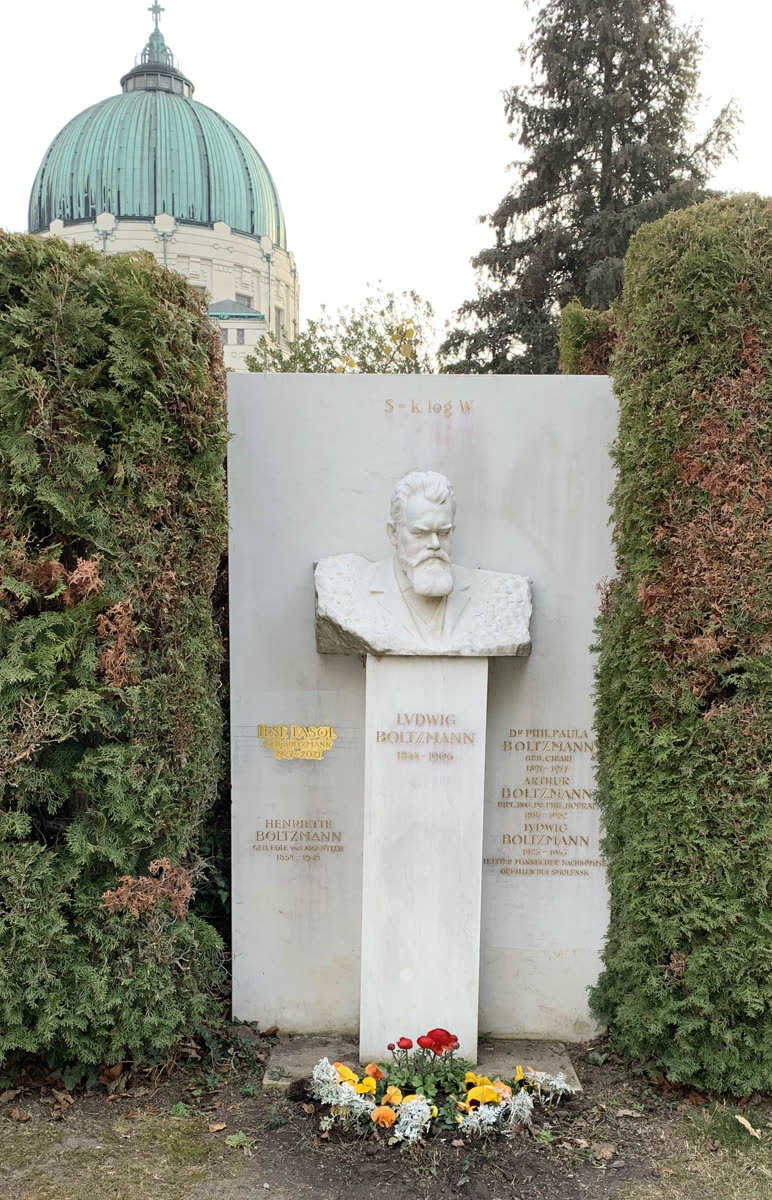
\includegraphics[width=\linewidth]{images/book4/boltzmann-grave.jpg}\par
{\footnotesize Makam Boltzmann.}
\end{minipage}
\end{history}

\section{Latihan}

\begin{exercise}[$\star$]\label{exo:b3:partition-functions:1}
Empat osilator berbagi empat kuantum. Daftarlah distribusi-distribusinya,
berikan bobot masing-masing, dan periksalah bahwa jumlahnya sama dengan
banyaknya cara menempatkan empat kuantum yang \omterm{def:b3:many-electron-atoms:indistinguishable}{tak terbedakan} pada empat
osilator, $\binom{7}{3}$. Distribusi mana yang paling mungkin?
\end{exercise}

\begin{exercise}[$\star$]\label{exo:b3:partition-functions:2}
Dua tingkat tak terdegenerasi berjarak \qty{2.5}{kJ/mol}. Hitunglah rasio
\omterm{def:b3:partition-functions:boltzmann}{populasinya} pada \qty{298.15}{K} dan pada \qty{1000}{K}. Berapakah limitnya
pada suhu yang sangat tinggi?
\end{exercise}

\begin{exercise}[$\star$]\label{exo:b3:partition-functions:3}
% ledger: aw:Ar
Hitunglah \omterm{def:b3:partition-functions:thermal-wavelength}{panjang gelombang termal} atom argon pada \qty{298.15}{K} dan fungsi
partisi translasinya dalam volume \qty{1}{dm^3}.
\end{exercise}

\begin{exercise}[$\star$]\label{exo:b3:partition-functions:4}
% ledger: diat:N2.Be, diat:N2.ae, diat:HCl.Be, diat:HCl.ae
Dengan $B_0 = \qty{1.990}{cm^{-1}}$ (\ce{N2}) dan \qty{10.440}{cm^{-1}}
(\ce{H^{35}Cl}), hitunglah $\theta_{\mathrm R}$ dan fungsi partisi rotasi suhu
tinggi setiap molekul pada \qty{298.15}{K}.
\end{exercise}

\begin{exercise}[$\star\star$]\label{exo:b3:partition-functions:5}
% ledger: diat:I2.we, diat:I2.wexe, diat:N2.we, diat:N2.wexe
Bilangan gelombang fundamental \ce{I2} dan \ce{N2} adalah \qty{213.27}{cm^{-1}}
dan \qty{2329.92}{cm^{-1}}. Hitunglah $\theta_{\mathrm V}$, $q^{\mathrm V}$ pada
\qty{298.15}{K}, dan fraksi molekul yang tidak berada pada $v = 0$.
\end{exercise}

\begin{exercise}[$\star\star$]\label{exo:b3:partition-functions:6}
% ledger: diat:NO.split, lev:Cl.2P1_2
Hitunglah fungsi partisi elektronik pada \qty{298.15}{K} untuk \ce{NO} (dua
\omterm{def:b3:quantum-model-systems:degenerate}{tingkat terdegenerasi} rangkap dua yang berjarak \qty{119.73}{cm^{-1}}) dan untuk
atom klorin (tingkat dasar ${}^2P_{3/2}$, ${}^2P_{1/2}$ pada \qty{882.35}{cm^{-1}}).
Berapa fraksi molekul \ce{NO} yang berada pada tingkat atas? Menuju apakah
$q^{\mathrm E}(\ce{NO})$ pada suhu tinggi?
\end{exercise}

\begin{exercise}[$\star\star$]\label{exo:b3:partition-functions:7}
Dari $q^{\mathrm T} = V/\Lambda^3$, turunkan energi dalam dan kapasitas kalor
pada volume tetap satu mol gas ideal monoatomik, lalu hitunglah $U - U(0)$
pada \qty{298.15}{K}.
\end{exercise}

\begin{exercise}[$\star\star$]\label{exo:b3:partition-functions:8}
% ledger: aw:Ar, s0:Ar_g
Gunakan persamaan Sackur--Tetrode untuk menghitung entropi molar standar argon
pada \qty{298.15}{K}; bandingkan dengan nilai tabel
\qty{154.846}{J.K^{-1}.mol^{-1}}. Seberapa besar perubahannya jika tekanan
dibagi 10?
\end{exercise}

\begin{exercise}[$\star\star$]\label{exo:b3:partition-functions:9}
% ledger: diat:HCl.Be, diat:HCl.ae
Hitunglah sumbangan rotasi pada entropi molar standar \ce{H^{35}Cl} pada
\qty{298.15}{K} ($\theta_{\mathrm R} = \qty{15.02}{K}$).
\end{exercise}

\begin{exercise}[$\star\star\star$]\label{exo:b3:partition-functions:10}
Dengan memperlakukan $J$ sebagai kontinu, tunjukkan bahwa tingkat rotasi yang
paling terpopulasi pada molekul linear terletak di dekat
$J_{\max} = \sqrt{T/2\theta_{\mathrm R}} - \frac12$. Hitunglah nilainya untuk \ce{HCl}
($\theta_{\mathrm R} = \qty{15.02}{K}$) dan \ce{CO} ($\theta_{\mathrm R} = \qty{2.766}{K}$) pada
\qty{300}{K}. Mengapa kedua cabang sebuah pita inframerah paling kuat beberapa
garis jauhnya dari pusat?
\end{exercise}

\begin{exercise}[$\star\star\star$]\label{exo:b3:partition-functions:11}
% ledger: diat:H2.Be, diat:H2.ae
Rumus Euler--Maclaurin memberikan $\sum_{J\ge0}f(J) \approx \int_0^\infty f(J)\dd J + \frac12f(0) -
\frac1{12}f'(0)$. Terapkan rumus itu pada $f(J) = (2J+1)\eu^{-\theta J(J+1)/T}$ dan
tunjukkan bahwa $q^{\mathrm R} \approx T/\theta +
\frac13$. Untuk suhu berapa $T/\theta$ tepat sampai 1\,\%? Apakah bentuk itu dapat
diterima untuk \ce{H2} ($B_0 = \qty{59.32}{cm^{-1}}$) pada \qty{298.15}{K}?
\end{exercise}

\begin{exercise}[$\star\star\star$]\label{exo:b3:partition-functions:12}
% ledger: diat:I2.we, diat:I2.wexe
Tunjukkan bahwa entropi molar vibrasi menuju nol jika $T \ll \theta_{\mathrm V}$ dan
menuju $R[1 + \ln(T/\theta_{\mathrm V})]$ jika $T \gg \theta_{\mathrm V}$. Hitunglah ungkapan
eksaknya dan limit ini untuk \ce{I2} ($\theta_{\mathrm V} = \qty{306.9}{K}$) pada
\qty{298.15}{K}, lalu berikan komentar.
\end{exercise}

\section{Soal: Menghitung Entropi Nitrogen}

\begin{problem}[{Soal akhir pekan --- menghitung entropi nitrogen: sumbangan
translasi, rotasi, vibrasi, dan elektronik pada entropi standarnya, yang
dihitung dari spektrumnya dan dibandingkan dengan tabel}]
\label{pb:b3:partition-functions:1}
% ledger: aw:N, diat:N2.Be, diat:N2.ae, diat:N2.we, diat:N2.wexe, s0:N2_g, const:h, const:kB, const:NA, const:c
Nitrogen adalah gas utama penyusun udara. Entropi molar standarnya pada
\qty{298.15}{K} dihitung di sini dari massa molarnya, \qty{28.014}{g/mol}, dan dari
tetapan-tetapan spektroskopinya: $B_e = \qty{1.998241}{cm^{-1}}$,
$\alpha_e = \qty{0.017318}{cm^{-1}}$, $\omega_e =
\qty{2358.57}{cm^{-1}}$, $\omega_ex_e = \qty{14.324}{cm^{-1}}$; suku dasar elektroniknya
adalah ${}^1\Sigma_g^+$. Tekanan standar $p^\circ = \qty{1}{bar}$;
$k = \qty{1.380649e-23}{J/K}$, $h = \qty{6.62607015e-34}{J.s}$.

\medskip\noindent\textbf{Bagian I --- Translasi.}
\begin{enumerate}[beginpenalty=10000]
  \item Hitunglah massa satu molekul.
  \item Hitunglah \omterm{def:b3:partition-functions:thermal-wavelength}{panjang gelombang termalnya} pada \qty{298.15}{K}.
  \item Hitunglah volume yang tersedia per molekul, $kT/p^\circ$.
  \item Simpulkan $q^{\mathrm T}/N$, dan berikan komentar tentang besarnya.
  \item Hitunglah entropi molar translasinya.
  \item Seberapa besar perubahannya pada setengah tekanan itu?
\end{enumerate}

\medskip\noindent\textbf{Bagian II --- Rotasi.}
\begin{enumerate}[resume, beginpenalty=10000]
  \item Hitunglah $B_0$.
  \item Hitunglah $\theta_{\mathrm R}$.
  \item Berikan \omterm{def:b3:partition-functions:symmetry-number}{bilangan simetrinya} dan jelaskan apa yang diperhitungkannya.
  \item Hitunglah $q^{\mathrm R}$ pada \qty{298.15}{K}.
  \item Apakah bentuk suhu tinggi dapat dibenarkan?
  \item Hitunglah entropi molar rotasinya.
  \item Dengan mengabaikan bobot spin inti, tingkat rotasi mana yang paling
        terpopulasi?
\end{enumerate}

\medskip\noindent\textbf{Bagian III --- Vibrasi dan keadaan elektronik.}
\begin{enumerate}[resume, beginpenalty=10000]
  \item Hitunglah kuantum vibrasi $G(1) - G(0)$.
  \item Hitunglah $\theta_{\mathrm V}$.
  \item Hitunglah $q^{\mathrm V}$ pada \qty{298.15}{K}.
  \item Berapa fraksi molekul yang berada pada $v = 1$?
  \item Hitunglah entropi molar vibrasinya.
  \item Berapakah sumbangan elektroniknya? Mengapa keadaan-keadaan elektronik
        tereksitasi dapat diabaikan?
\end{enumerate}

\medskip\noindent\textbf{Bagian IV --- Jumlah dan perbandingan.}
\begin{enumerate}[resume, beginpenalty=10000]
  \item Jumlahkan sumbangan-sumbangan itu.
  \item Bandingkan dengan nilai tabel \qty{191.609}{J.K^{-1}.mol^{-1}}.
  \item Pada pengukuran apa nilai kalorimetri dalam tabel bersandar?
  \item Mengapa tabel dapat mengabaikan spin inti?
  \item Nyatakan hasilnya: entropi molar standar nitrogen pada
        \qty{298.15}{K} yang dihitung dari tetapan-tetapan spektroskopinya.
\end{enumerate}
\end{problem}
